\chapter{绪论}

\section{研究背景与研究意义}
\label{sec:research_background}
随着社会的发展,人民生活和现代化水平的不断提高,导致对电能的需求越来越大,电力系统作为维持国计民生的重要组成部分,其稳定运行、经济性、可靠性以及安全性越来越重要。
近年来,随着电力系统规模的不断扩大和其复杂性的逐步增加,电力系统各元件之间的关联越来越紧密。电力系统在促进社会发展和人民生活水平提高的同时,由于某一局
部故障而导致电网的连锁性崩溃,甚至导致大停电事故的例子屡见不鲜,从这方面来讲,这些电网故障不仅带来巨大的经济损失,还将严重影响社会经济的发展和人民的生活水平的提高。

自进入21世纪后,全球各地发生了很多大面积电网瘫痪事故。在国内,2008年南方特大雪灾导致的全国大范围停电事故对社会经济和人民生活造成了极大的影响,我国遭遇了50年一遇的
冰雪灾害,由于暴雪、冻雨导致华南地区、华中和华北部分地区输变电线路出现大范围断线倒塔,造成大范围停电限电,严重影响了电网安全运行,有地区甚至断水断电十余天,
引发了交通运输、物资调度等方面的连锁反应,严重影响了人们的日常生活,影响人数达2亿人。据调查统计,此次灾害导致停运电力线路37606条,停运的变电站共2027座,
111--500~kV线路倒塌8165座,给南方地区造成了巨大的经济损失。
在国外,2018年3月21日,巴西电网发生大面积停电事故,涉及巴西北部与东北部14个州,其中受影响最为严重的是贝里奥格兰德州、帕拉伊巴州和马拉尼昂州。在此次停点事故中,北部
和东北部电网与主网裂解,最终损失负荷21735~MW,相当于巴西互联电网停电前负荷的27\%,全国约四分之一的用户断电。事故原因为巴西欣古换流站交流测500~kV断路器故障\cite{refs1}。
此外,近期发生的“3.7”委内瑞拉停电事故,委内瑞拉政府称电力系统遭到三个阶段的攻击,分别是网络、电磁和人为破坏的攻击,其攻击的方式都是使电力系统的中枢节点故障,从而引发
电力系统连锁故障。在此次停电事故中,委内瑞拉23个州中,一度有20个州全面停电,造成大规模交通拥堵,学校、医院、工厂、机场等都受到严重影响,给人们带来巨大恐慌。

在世界范围内,电力系统大停电事故时有发生,已逐渐得到人们的重视。国内外学者开始研究停电事故的原因以及如何降低其发生的概率,电网脆弱性的研究也越来越成为专家学者研究的
热门领域。从大多数停电事故的原因可以看出:电网大面积瘫痪之初,都是某一元件的局部故障所引起的,由于电网的级联特性,电网的故障范围不断扩大,最终导致大面积停电事故发生。
导致元件局部故障因素有很多,比如外部环境的变化、网络攻击以及人为操作等,电力系统在运行过程中,脆弱性是电力系统固有的属性,当这些扰动因素作用于电力系统时,电力系统的
脆弱性显现的概率会大增,其自身潜在的脆弱性会对其安全可靠运行造成严重威胁,因此有必要对电力系统进行脆弱性分析,研究其脆弱性指标,并建立量化评估模型,进一步识别系统的
脆弱环节,为电力系统设计和维护人员提供可靠安全的防护方案,从而降低电力系统发生故障的概率。
\section{国内外研究现状}
\label{sec:research_presentSituation}

\subsection{脆弱性研究起源及现状}
\label{sec:origin}
脆弱性,这一概念在医学领域中被最早提出,在流行病学\cite{refs2,refs3}中,研究的是某些地区更容易发生流行病,或人体的哪些部位更容易被细菌或病毒感染。
在心脑器官领域中,研究的是不同药物或治疗方案对心脑血管以及其他脏器的耐受程度\cite{refs4,refs5}。自20世纪70年代后,专家学者开始将脆弱性概念用于生态系统领域\cite{refs6,refs7}。
80年代后,脆弱性逐步扩展到自然灾害和全球气候变化中,并逐步在可持续发展的研究中频繁出现,进入21世纪,脆弱性的研究逐渐延伸到社会经济体系、计算机网络、工业控制系统以及
电力系统领域。

“脆弱性”概念早在20世纪60年代就已提出,在之后很长时间一直用于环境科学,医学以及人文科学。脆弱性领域的研究覆盖多个学科,不同领域对脆弱性现象的研究侧重点不同,到目前为止,还没有
一个公认的脆弱性概念。20世纪70年代起,一些生态环境研究者开始研究生态领域的脆弱性现象,学者M.Pacifici分析研究了气候变化对生态系统中物种多样性带来的脆弱性影响,他对脆弱性的
理解是气候变化对生物种类的影响程度,并建立了三种评估气候脆弱性的模型\cite{refs8}。在1991年,美国和前苏联建立了生态脆弱性的评价方法与评价因子,对生态脆弱性的起因、脆弱程度
以及相关的补偿机制开展了大量实验研究\cite{refs9}。在经济学领域中,经济学家认为脆弱性是对于未知情况的可能性或不确定性,具体指的是系统受到不利因素或者受到损害的可能性或不确
定性\cite{refs10,refs11}。金融学家Minsky在1982年提出的“金融脆弱性假说”为金融脆弱性理论研究提供了分析框架\cite{refs12},之后Diamond和Dybvig提出了“预期自致型理论”和“安全边
界说”\cite{refs13},这三个理论分别从投机、信心、银行资产质量等方面阐述了银行脆弱性生成机理。直到1990年以后,脆弱性概念逐渐进入工程研究领域,1997年,
LH.Keel和SP.Bhattachacharyya对$H_{2}$、$H_{\infty}$以及$l$等鲁棒控制器组成的控制系统进行研究,发现优化后的闭环控制系统在特定外部扰动的作用下极易产生不稳定的状态,其稳定
裕度指标很差,于是采用了“脆弱性”概念来描述控制系统这种隐形特性\cite{refs14}。在网络安全领域中,国内外专家们对网络脆弱性评估技术进行了深入的理论研究和实际应用,提出了一系列
的评估模型,主要有定性、定量、基于规则和基于模型等评估方法,还有后来发展的动态和分布式评估方法\cite{refs15,refs16}。

在国内,中国学者对脆弱性理论的研究相较于国外较晚,脆弱性概念最早出现在计算机网络领域\cite{refs17},在全球化趋势下,中国社会经济快速发展,各个领域的矛盾和摩擦层出不穷,
中国学者对脆弱性的研究领域不断扩展,研究方法不断深入,在生态系统\cite{refs18,refs19}、气候变化\cite{refs20,refs21}、金融机构\cite{refs22,refs23,refs24}、信息安全
\cite{refs25,refs26}、交通运输\cite{refs27,refs28}等方面进行了广泛的研究。在脆弱性理论和研究方法上,也不断进行研究和探索,目前国内学者普遍认为脆弱性是系统本身固有的一种
属性,由于系统本身对扰动有一定的敏感性,不同的系统对扰动作用后的恢复能力不同,只有在内部或外部扰动作用下,系统脆弱性才可能显现。在研究方法上,主要以研究脆弱性指标\cite{refs29},
脆弱性指标融合方法\cite{refs30},脆弱性评估模型为主。近年来,在电力系统研究领域,复杂网络理论\cite{refs31}受到了越来越多学者的重视,并以此为基础对电力系统建模以及脆弱性
指标的研究,从而综合分析电力系统脆弱性。


\subsection{电力系统脆弱性研究综述}
\label{sec:presentPowerSys}
电力系统是由发电厂、送变电线路、供配电所和用电负荷等环节组成的电能生产与消费系统。电力系统脆弱性是近年来针对电力系统安全性和可靠性提出的一个新概念,目前还没有公认的定义和统一的
分析标准。但从已有的参考文献看,电力系统脆弱性是用来描述系统在正常运行情况或各种随机因素的作用下,系统承受干扰或故障的能力及系统不能维持正常运行的可能趋势及其影响\cite{refs32}。
有学者将引起系统脆弱性显现的不确定因素成为脆弱源,比如气候变化、地理、认为破坏等因素,将系统内部某些易发生故障的环节称为系统脆弱点。

通过查阅大量的参考文献后,对电力系统脆弱性的研究内容分为以下四类:
\begin{itemize}
  \item 电力系统脆弱性研究理论与方法
  \item 电力系统脆弱性评价指标和融合方法的研究
  \item 针对电力系统评价指标建立系统评价模型,并系统进行脆弱性分析
  \item 根据系统脆弱性评价结果提出相应的安全管理机制与应对策略 
\end{itemize}

在电力系统脆弱性理论研究方面,复杂网络是把一个复杂系统抽象为网络,将复杂系统内的元件视为网络的节点,将元件之间的联系视为连接网络中各个元件的边,由此建立复杂网络的模型。在此模型
基础上,从复杂网络的拓扑模型出发,运用图论、统计学理论对整个复杂网络进行局部、全局的研究,经过二十多年的发展,复杂网络的建模和分析方法,可用于描述系统内各个元件的相互关联以及系
统的整体描述,并且该理论和其研究方法已越来越多应用于各个领域,比如社会关系网络\cite{refs33}、交通运输网络\cite{refs34,refs35,refs36}、航空海运网络\cite{refs38,refs39}、电力
系统网络\cite{refs40,refs41}等,大多数复杂网络的复杂性的特征为:网络规模庞大、连接结构的复杂性、节点的复杂性、网络时空演化过程复杂、多重复杂性融合等,电力系统作为最复杂、最广泛
的人造技术网络,具有以上复杂网络的特性。在二十多年的发展中,复杂网络理论已成为电力系统研究领域中最具权威性的理论。

在电力系统脆弱性评价指标研究方面,通过参考大量文献研究后,主要分为两个方面进行研究分析,从电力系统拓扑结构来讲,主要基于复杂网络理论来进行研究,复杂网络的结构特征参数的统计描述有:
平均路径长度、节点度、聚类系数、介数、网络冗余、网络结构熵、系统全局效能等。通过复杂网络理论对系统进行建模,在复杂网络的特征参数的基础上,进行电力系统结构脆弱性指标的研究。
从电力系统运行状态来讲,主要是基于裕度、灵敏度、能量函数这三个方面进行指标研究,裕度法主要是通过比较电力系统当前运行状态点与临界点的裕度指标来评估节点的脆弱性\cite{refs42,refs43,refs44};
灵敏度法是主要是采用灵敏度分析法,通过改变某一变量研究其对其它系统变量的影响程度来评估系统的状态脆弱性\cite{refs45,refs46};能量函数法是通过能量函数表达式对支路或节点的状态脆弱性
进行评估,其考虑的是系统的暂态脆弱性\cite{refs47,refs48,refs49}。以上三种方法可由能量裕度、节点电压、系统频率、节点功率以及发电机功角等状态量为基础指标进行进一步研究分析。

在电力系统量化评估研究方面,基于复杂网络分析评估法、基于暂稳脆弱性评估法和基于概率风险的脆弱性评估法是三类常用的方法。基于复杂网络分析评估法是以复杂网络为基础,从网络拓扑结构分析连锁
故障的传播机理\cite{refs50,refs51,refs52};基于暂稳脆弱性评估法主要研究的是电力系统在暂态过程中是否能够保持在稳定的状态,此类方法主要包括基于暂态能量函数的脆弱性评估\cite{refs53}
和基于关键割集法的脆弱性评估方法\cite{refs54};基于概率风险的脆弱性评估法中有确定性评估法\cite{refs55}、概率性评估法\cite{refs56}、风险评估法\cite{refs57},此外基于蒙特卡洛法进行
脆弱性评估\cite{refs58}也是比较常用的,这些方法大多采用的是概率统计的方法对系统进行脆弱性评估。在系统脆弱性指标融合方法的研究中,可以参考与改进的主要领域在多属性决策方面,主要分为
主观、客观和组合赋权三个方面,主观评价方法有层次分析法、模糊层次分析法、专家调查法和环比评分法等;客观评价法主要有离差最大化法、熵信息法、基于方案满意度法、基于方案贴进度法等;组合赋权
法是指将不同赋权法所得到的权重系数按照一定的方法进行组合\cite{refs59}。

通过建立电力系统的评估模型,可根据融合指标值对电力系统的节点或支路的脆弱性等级进行划分,根据节点或支路的脆弱性等级,对电力系统采取相应的安全管理机制与应对策略,从而减低电网连锁故障发生
的概率,保障用电安全。



\section{研究内容与研究路线}
\label{sec:research_curise}

\subsection{待解决的问题}
\label{sec:research_problem}
对于电力系统的脆弱性分析与量化评估的研究至今依然存在很多待解决的问题,如:
\begin{enumerate}[(1)]
  \item 脆弱性概念虽然很早就已经提出,但对于电力系统的脆弱性描述和定义尚不清晰,缺乏全面性;
  \item 电力系统中的脆弱性研究的研究理论与方法虽然比较权威和可行,但是在脆弱性指标研究方面,大多数论文只从单一方面进行研究分析,评价指标缺乏全面性;
  \item 在很多电力系统脆弱性研究中,并未明确脆弱性研究的关键问题,研究对象和指标基于整个系统,对系统整体脆弱性进行评估,而非研究和识别系统的脆弱环节;
  \item 在指标融合方法上,虽然各个研究领域的指标融合方法各有千秋,但对于在电力系统的指标融合方面的考虑不够合理全面;
  \item 对于电力系统脆弱性量化分析与研究,脆弱性量化评估模型的相关研究未形成严格的理论体系。
 \end{enumerate}

\subsection{研究内容与章节划分}
\label{sec:contendAndIdea}
本文针对电力系统脆弱性分析与量化评估研究中待解决的问题,在研究了复杂网络与电力系统之间的关联的基础上,给出了较为科学合理的电力系统脆弱性定义。并进一步对电力系统从结构和状态两个方面分别
给出结构脆弱性和状态脆弱性的定义与数学描述,使得电力系统的脆弱性概念更为全面。根据结构脆弱性和状态脆弱性的理论研究进行脆弱性指标选取,从而建立系统脆弱性综合评估指标集。分别对一级脆弱
性指标和二级脆弱性指标进行权重分配、指标融合建立了电力系统脆弱性量化评估模型。并且以$IEEE39$系统数据为例进行电力系统的脆弱性分析与量化,识别系统的脆弱环节。本文的章节安排如下:

第~1~章~:查阅国内外“复杂网络”、“脆弱性分析”等相关领域研究文献与论文,对脆弱性概念的起源与发展以及脆弱性在电力系统的研究现状做了详细的调研与综述,在明确研究方向和理论依据的基础上,
科学提炼出待解决的问题,确定研究方法、目标和技术路线。
%为后续研究电力系统脆弱性与量化分析方法提供必要的理论依据。

第~2~章~:本章基于复杂网络理论,阐述复杂网络的概念和特征参数,通过MATLAB仿真实验验证电力系统的小世界性和无标度性,并通过对复杂网络脆弱性概念的描述,明确电力系统脆弱性研究的关键问题。
%研究分析复杂网络理论的相关概念,对复杂网络的定义与数学描述进行分析,以此为基础建立电网模型。在研究复杂网络的基本特征参数的同时,为后续第三章提出结构脆弱性指标提供理论依据。
%在分析复杂网络定义与特性的基础上,进一步分析研究复杂网络的脆性理论,分析整个复杂系统的脆弱性指标,为后续第五章的电力系统结构脆弱性仿真实验分析打下基础。为了验证电力系统的网络特性,
%本章还研究分析了复杂网络的小世界模型和无标度模型。

第~3~章~:通过研究分析电力系统稳定性、可靠性、鲁棒性之间的区别与联系,得出电力系统脆弱性的本质并进行脆弱过程和数学描述;分别从电力系统结构和状态两个方面对脆弱性的理论分析方法进行研究,
提出脆弱性指标。结构脆弱性方面,侧重于系统保持其结构完整性的能力,研究系统在扰动作用下系统受影响的程度,状态脆弱性方面,专注于在系统的抗干扰能力,建立负荷模型,结合蒙特卡洛模拟方法,
并以此作为状态脆弱性仿真分析的基础。

第~4~章~:针对结构脆弱性与状态脆弱性,分别根据各自脆弱性的定义与特征选取能够反映其脆弱现象的评价指标,结合并改进客观评价法及多指标融合法,建立了电力系统脆弱性量化评估的数学模型。解决
系统脆弱性现象难以量化的问题,为后续量化评估电力系统脆弱性问题提供了理论参考。

第~5~章~:以$IEEE118$电力系统为例,在系统模型建立的基础上,研究不同攻击策略对电网拓扑结构完整性及系统性能的影响程度;以$IEEE39$电力系统为例,分析不同指标对系统结构和状态的影响,
采用多指标融合方法分别得到结构和状态脆弱性指标,分别分析各系统节点的结构脆弱性和状态脆弱性,基于D-S证据理论得到系统的综合脆弱性模型,基于脆弱性量化评估模型对电力系统节点脆弱性进行等级划分,
进一步量化分析电力系统节点的脆弱程度,得出脆弱性评估结果为后续安全管理机制与应对策略提供了理论依据。

第~6~章~:总结本文的研究工作,对本文中电力系统脆弱性分析与量化数学模型的优点和不足进行了详细的阐述,并为后续研究工作提出了若干点建议与展望。

通过以上的研究工作,完成电力系统脆弱性分析与量化评估的理论研究及实验验证与分析,具体的技术路线图如下所示。
\begin{figure}[H] % use float package if you want it here
  \centering
  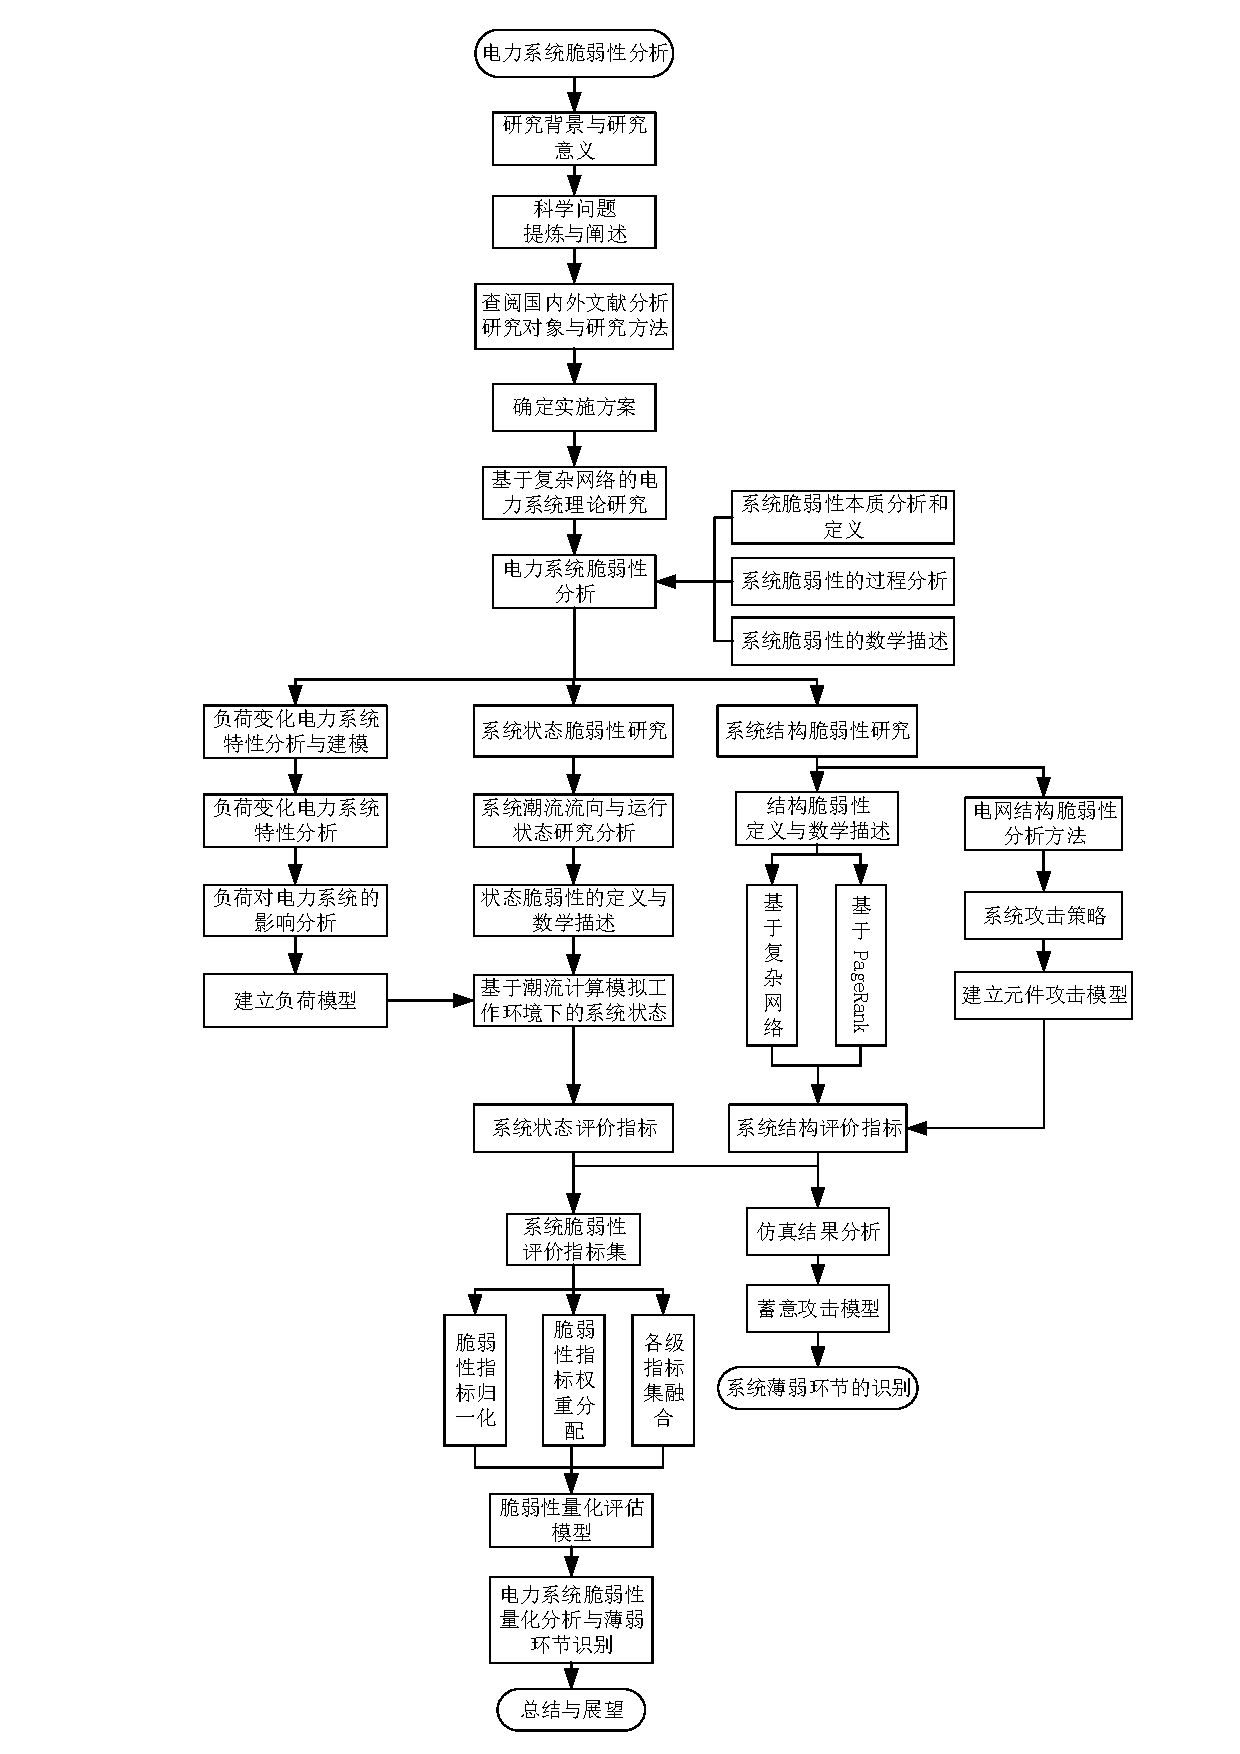
\includegraphics[height=23cm]{technicalRoute.pdf}
  \caption{技术路线图}
  \label{fig:technicalRoute}
\end{figure}
